% TODO:
%   - Title spelling etc
%   - Kijk na of titels in header overflowen
% ----------  
% Questions:
%   - XXX

% technology readiness level bespreken?

% Cohen's kappa value

% Uncomment this if the use of parts is desired
\part{Reflection on the results of this master thesis}
\label{part:reflection}

% Will need a new title since it is no longer a system to use
\chapter{Evaluation of the proposed pipelines}
\label{ch:evaluation}

% ---------------------------------------------- 
% INTRODUCTION
% ---------------------------------------------- 
\section{Introduction to this chapter}
\label{sec:evaluation_introduction}
% NOTE: "Introduction" exists in each chapter and gives a short intro to the chapter + what can be expected in the chapter

The previous chapters discussed in great detail which \gls{mi} \gls{eeg} classification pipelines were considered for this master thesis, how they work and how they can be evaluated.
This chapter details the performed evaluations and the results obtained.
In particular, three main test settings were used: intrasession, intersession and intersubject evaluation.
Besides providing an overview of the obtained evaluation metrics, reasoning into why certain experiments were performed and why certain results were expected are also given.
The used open-source \gls{mi} \gls{eeg} dataset is also briefly discussed.
Most experiments revolve around offline \gls{mi} \gls{eeg} classification performance, as this is the focus of this master thesis.
Some pilot experiments regarding recommended changes for going to an online setting discussed in Chapter \ref{ch:online_bci_system} were also performed and are also discussed in this section.

% ---------------------------------------------- 
% USED DATA
% ---------------------------------------------- 
\section{Three class MI EEG data source}
\label{sec:evaluation_data_source}

Following this master thesis' proposal of splitting \gls{bci} development in at least four distinct papers, as discussed in Section \ref{subsec:bci_opportunities_obstacles_lack_of_testing}, this master thesis focusing on the classification pipeline should provide a summary of the data used.
The \gls{mi} \gls{eeg} data used for this master thesis is from an open-source dataset by \citet{eeg_data}.
The complete dataset provided by them consists of four different types of \gls{mi} interaction tasks, of which this master thesis works with the three class \gls{mi} \gls{eeg} dataset provided as the "CLA" dataset.

The hardware used for the data acquisition of this dataset uses the international 10-20 system discussed in \ref{subsec:biomedical_signals_working_with_eeg_standards}.
The used \gls{eeg} equipment makes use of wet electrodes and a sampling rate of 200\gls{hz}.
The participants were seated in a comfortable position throughout the experiment and remained motionless throughout the recordings, with a fixed gaze-fixation point to limit the presence of muscle artefacts who were discussed in Section \ref{subsec:biomedical_signals_working_with_eeg_artefacts}.
The provided data is band-pass filtered to include the frequencies between 0.53\gls{hz} and 70\gls{hz}.
A band-stop filter was also in place to remove \gls{ac} artefacts as discussed in Section \ref{subsec:biomedical_signals_working_with_eeg_artefacts}.
All of these frequency filters are hardware filters directly integrated into the hardware of the EEG-1200 hardware used for data acquisition.

The recordings of the CLA dataset provides balanced sampels of three \gls{mi} tasks reffered to as left-hand \gls{mi}, right-hand \gls{mi} and neutral \gls{mi}.
For the left-hand and right-hand \gls{mi} tasks, the participants were asked to imagine closing and opening the respective fist once.
For the neutral \gls{mi} task, the patient was asked to perform no \gls{mi}.
The communication of which task to perform was done via a simple graphical interface.
Upon showing the icon for which task to perform (event onset), the subject should perform the specific \gls{mi} task.
The icon is visible on the screen for one second past the event onset.
A random resting period of 1.5 to 2.5 seconds was present between the event offset and the event onset of a new task.
This process was repeated for 15 minutes, after which a longer resting period was present where it was ensured the \gls{eeg} equipment remained properly seated.
In total, three 15-minute trials were performed in one session.
This resulted in roughly 300 samples for each \gls{mi} task for each session.
Some subjects only had one recorded session whilst others had up to three.
All subjects were healthy, between 20 and 35 years old and living in Turkey.
No specific survey was performed to test the \gls{mi} capabilities beforehand nor does \citet{eeg_data} describe that any specific \gls{mi} training happened.

The data from the CLA dataset is provided as MatLab files originally.
To make them usable in Python, the experimental notebooks provided on the GitHub repository of this project provide conversion methods to convert these MatLab files to MNE Raw objects \citep{github_project, mne}.
To facilitate the use of this dataset in Python for other researchers, the GitHub repository provides the CLA dataset as \gls{fif} files \citep{github_project}.
These \gls{fif} files can be easily opened with MNE Python and include all provided details by \citet{eeg_data} stored in the associated info object.
The utility file $\texttt{CLA\_dataset.py}$ provides many functions for working with this CLA dataset in Python.

% ---------------------------------------------- 
% GENERAL REMARKS
% ---------------------------------------------- 
\section{General remarks on experiment setups}
\label{sec:evaluation_general_remarks}

To provide the best possible reproducibility all resources needed to recreate the experimental results are available on the documented GitHub repository of this master thesis \citep{github_project}.
This includes saved weights of the exact models used for the results discussed in this chapter and many utility files to facilitate loading and working with these models.
As discussed, the used data is also provided as MNE Raw objects and stored as \gls{fif} files.

All training and testing was done on a 64-bit Windows 10 Pro machine with an Intel Core i5-4690K overclocked at 4.2GHz.
An MSI NVIDIA GeForce GTX970 \gls{gpu} was used in the training of the \gls{dl} models with CUDA support through the CuDNN 8.2.2 driver.
The system in question had 16GB of ram, of which an approximate 10GB was usable for the training procedure.
These specifications allowed for sufficient training of the two-step \gls{ml} and state-of-the-art \gls{cnn} models in a reasonable time.
The longest cross-validated grid search hyperparameter tuning experiment for the two-step \gls{ml} approaches took around 30 hours to finish.
The longest experiment for the literature proposed \gls{cnn} models was finished in less than 6 hours.
The \gls{lstm} models were computationally heavy, and the convolutional \gls{lstm} extension to EEGNet does not have CUDA support.
This resulted in longer training times, with manageable times of under 6 hours for the regular \gls{lstm} extended EEGNet model.
However, for the convolutional \gls{lstm} extend EEGNet model, certain configurations were not possible due to limited video RAM and fewer epochs were performed for training.
The latter didn't seem to influence the results as the evolution of both training and validation accuracy and loss converged in all experiments.

The used representation of the \gls{eeg} signal provided through MNE makes use of extremely small values.
Whilst this was not an issue for the traditional two-step \gls{ml} approaches due to the use of \gls{csp} functionality provided by the same library, it did cause training issues for the \gls{dl} approaches.
To combat this, all data used for the \gls{dl} approaches was first multiplied by 1000000.

Each experiment made use of a fixed length window around a known event as described in Section \ref{subsec:processing_signals_general_pipeline_windowing}.
Two window lengths were considered, a 0.5-seconds window used for all experiments and a longer 1.5-second window additionally tested for most experiments.
The 0.5 seconds window started 0.1 seconds after the event onset and ended 0.6 seconds after the event onset.
The 1.5 seconds window started 0.25 seconds before the event onset and ended 1.25 seconds after the event onset.

The traditional two-step \gls{ml} approaches made use of cross validated gridsearch hyperparameter tuning to find the best possible combination of parameter settings, as discussed in Section \ref{subsec:offline_bci_system_two_step_ml_basic_csp}.
Due to the computational power that would be needed to perform such a cross-validated grid search for hyperparameter tuning of the \gls{dl} methods, parameters were chosen based on the literature proposed configurations and finetuned based on pilot studies performed in the experimental notebooks.
This also means that whilst the traditional two-step \gls{ml} approaches mostly have 4-fold evaluation accuracy reported together with their standard deviation, the \gls{dl} models only have a singular evaluation accuracy available obtained from a typical 20\% split during Keras training.

The \gls{dl} models were trained for sufficient epochs, 250 to 2500 dependent on the data and pipeline, where both training scores and validation scores on basis of accuracy and loss were monitored to ensure stable training.
For each training procedure of the \gls{dl} models, two variants of the model were saved.
One where the validation loss was lowest and one where the validation accuracy was the highest.
These variants are used for obtaining the final results on the test sets, which were equal for all models and 20\% of the total available data.
The best variant of these two is the one reported in this chapter.
Due to the use of balanced data, the accuracy of a random model would be $\frac{1}{3}$ in all experiments.

\begin{figure}[ht]
    \centering
    \begin{subfigure}{0.9\textwidth}
        \centering
        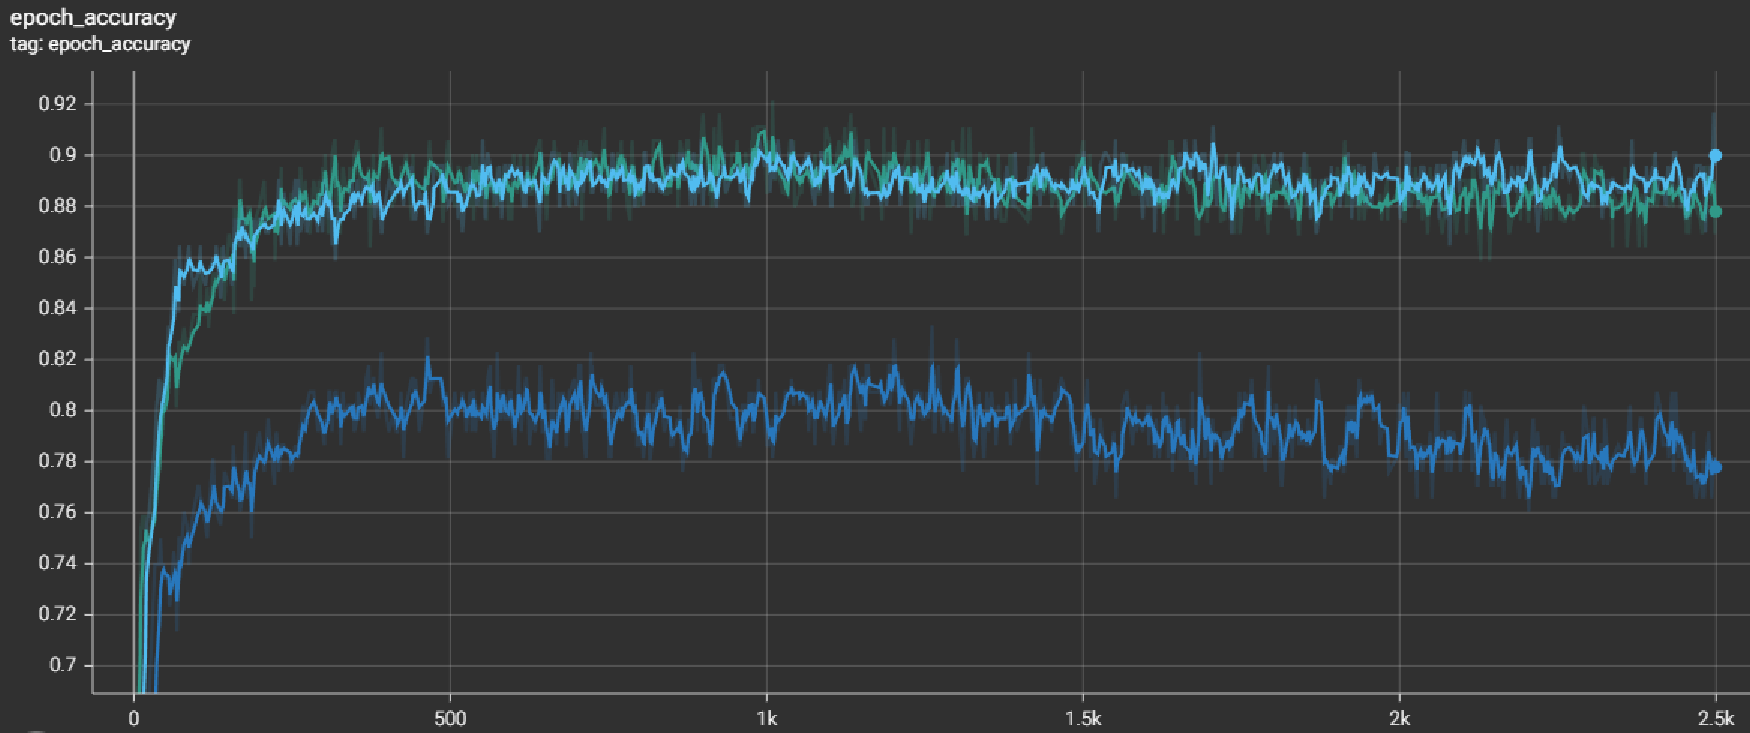
\includegraphics[width=\textwidth]{../images/results/accuracy.pdf}
        \captionsetup{width=\linewidth}
        \captionsetup{justification=centering}
        \caption{Evolution of validation accuracy over time.}
        \label{fig:results_tensorboard_acc}
    \end{subfigure}
    \hfill
    \vfill
    \begin{subfigure}{0.9\textwidth}
        \centering
        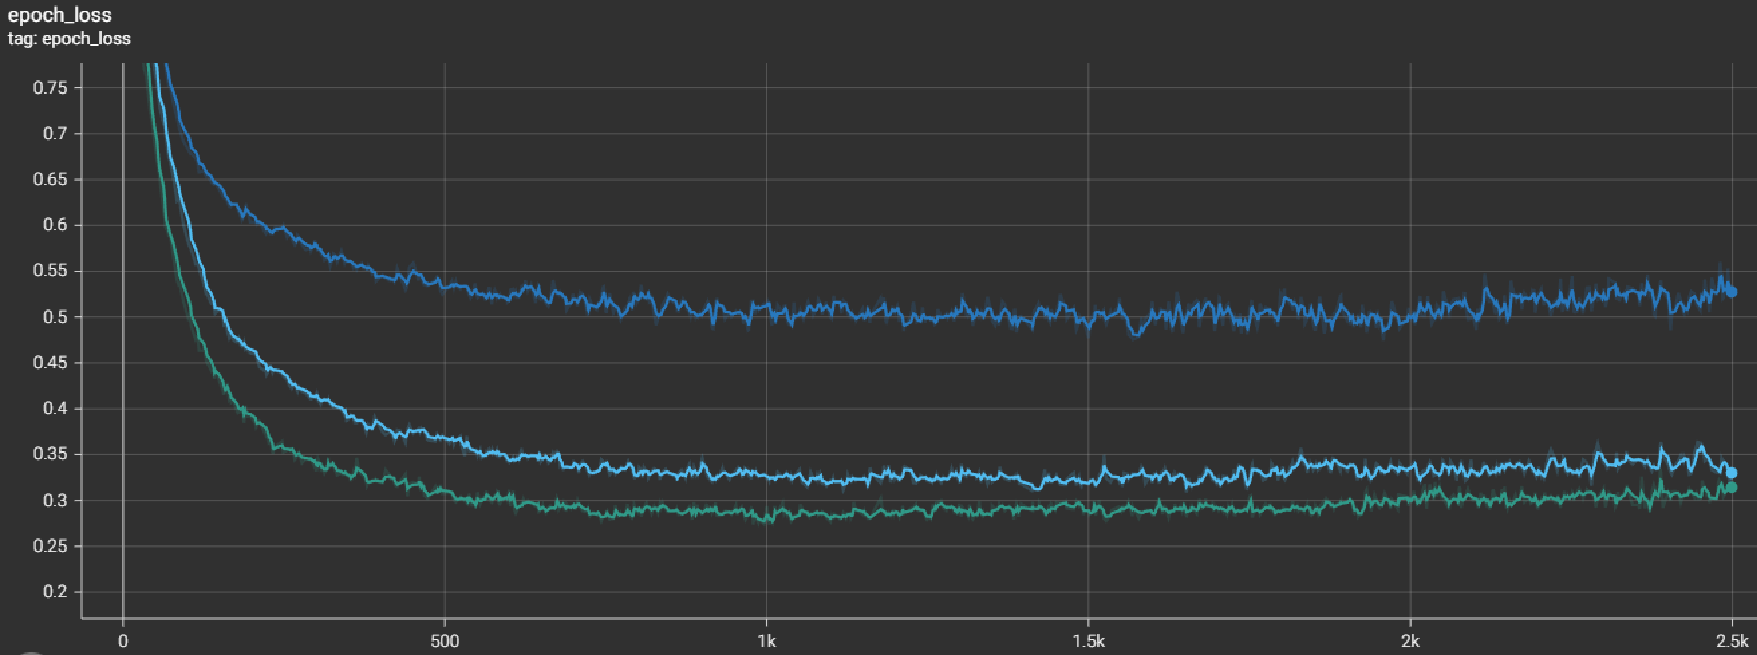
\includegraphics[width=\textwidth]{../images/results/loss.pdf}
        \captionsetup{width=\linewidth}
        \captionsetup{justification=centering}
        \caption{Evolution of validation loss over time.}
        \label{fig:results_tensorboard_loss}
    \end{subfigure}
    \captionsetup{width=\linewidth}
    \captionsetup{justification=centering}
    \caption{Evolution of both validation accuracy and validation loss over time. Graphs shown are from the intrasession experiment of EEGNet for subjects B (dark blue), C (light blue) and E (green). The time axis denotes the epoch in which the result is obtained.}
    \label{fig:results_tensorboard}
\end{figure}

These general remarks should suffice for a precise understanding of the results discussed in the remainder of this chapter.
As discussed, all learned models and the code for all performed experiments is available on the GitHub repository of this master thesis to ensure complete reproducibility \citep{github_project}.

% ---------------------------------------------- 
% CONSIDERED EVALUATION METRICS
% ---------------------------------------------- 
\section{Considered evaluation metrics}
\label{sec:evaluation_eval_metrics}



% ---------------------------------------------- 
% INTRA SESSION
% ---------------------------------------------- 
\section{Intrasession evaluation}
\label{sec:evaluation_intrasession}


\begin{figure}[ht]
    \centering
    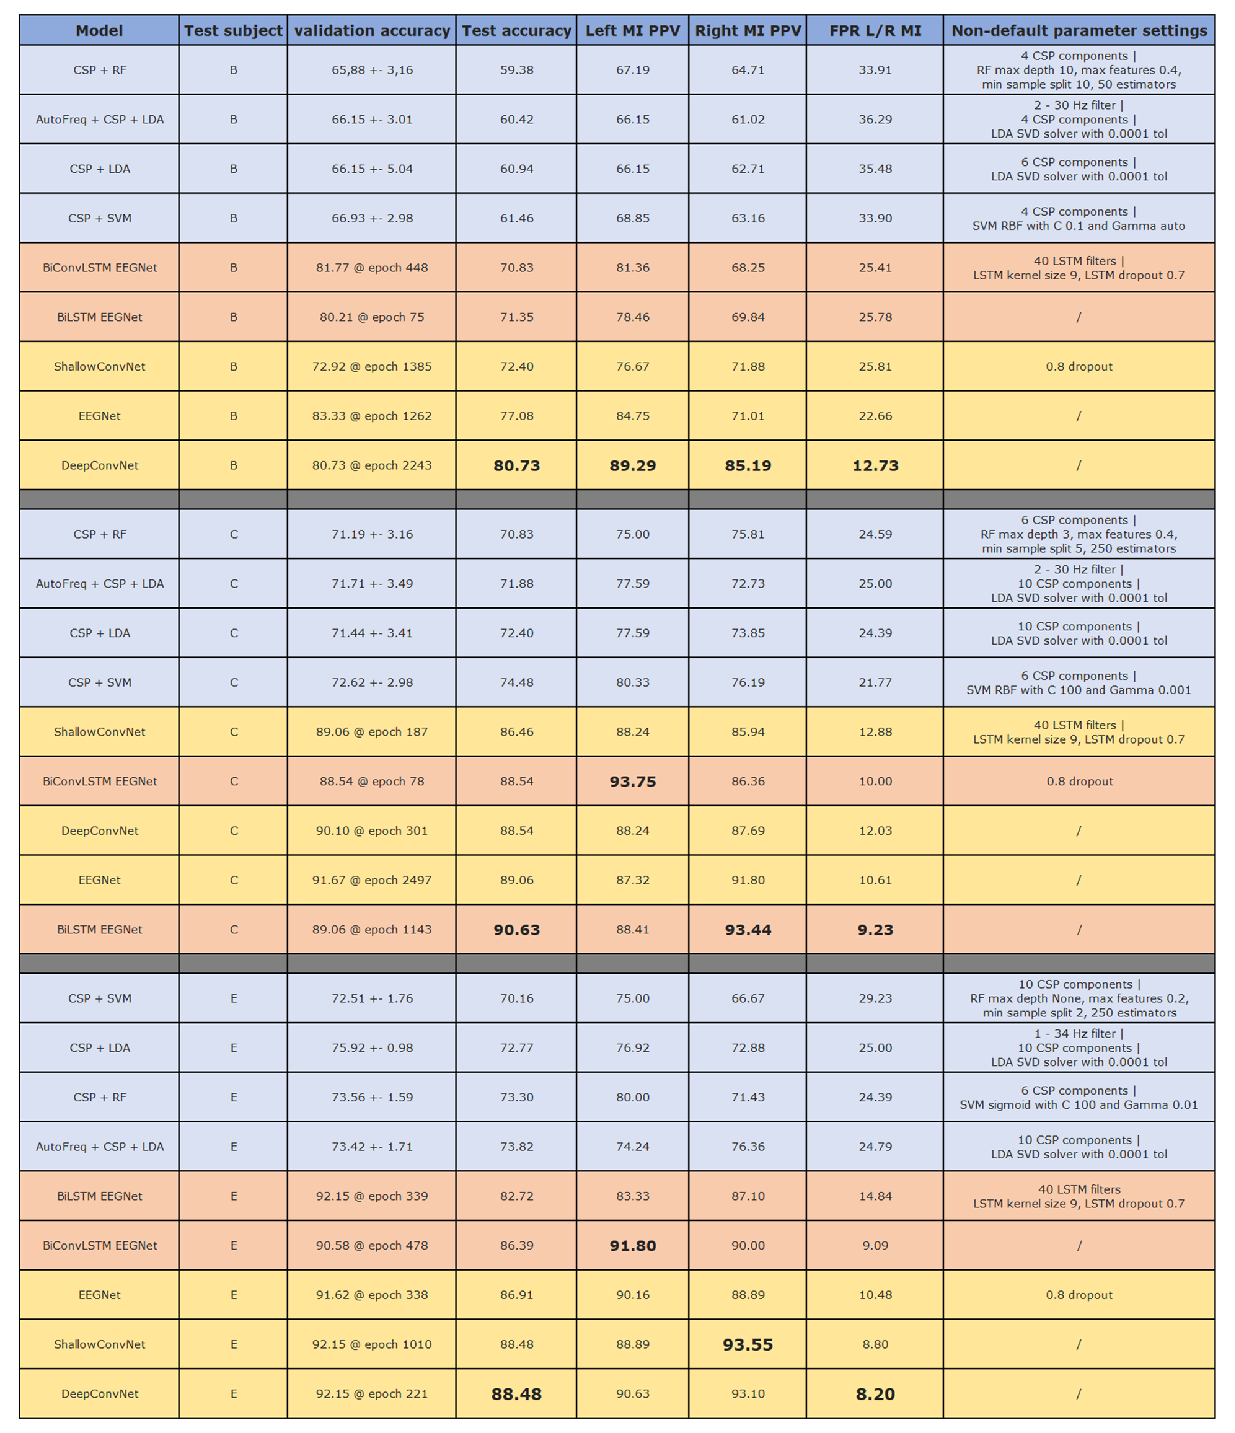
\includegraphics[width=\linewidth]{../images/results/intrasession.pdf}
    \captionsetup{width=\linewidth}
    \captionsetup{justification=centering}
    \caption{Intrasession results for all classification approaches. Results are sorted based on the test subject and the obtained classification result on the test set. Colorcodes denote either two-step \gls{csp} approaches, literature proposed \gls{cnn} approaches or master thesis proposed \gls{cnn}-\gls{lstm} approaches} 
    \label{fig:results_intrasession}
\end{figure}


The first experimental setup consisted of an intersession evaluation.
In an intrasession setting, the model is trained and tested on \gls{mi} \gls{eeg} data from the same subject and from the same session.
This experimental setup is the easiest to learn as it is least influenced by the generalisability issues of \gls{mi} \gls{eeg} data discussed in Section \ref{subsec:biomedical_signals_working_with_eeg_generalisation}.
The models are trained on 60\% of the data, validated on 20\% of the data for finding the best parameter configurations and tested on the test set consisting of 20\% of the data.
The validation accuracy was determined on both validation and test set.
The tests are identical between all experiments on the same subject.
The two-step \gls{ml} approaches used 4-fold cross-validation gridsearch for finding the optimal parameters based on validation accuracy.
The used folds where identical between all experiments due to a set random seed.
The one-step \gls{dl} approaches all made use of the same validation and train split.


Figure \ref{fig:results_intrasession} summarizes all obtained results in terms of validation and test accuracy for the experiments of this type.
From these results it becomes appearant that the \gls{cnn}-\gls{lstm} approaches have no real performance gains or decrease compared to the EEGNet model it is based on.
One exception is the results for subject B where the \gls{cnn}-\gls{lstm} approaches perform worse then EEGNet.
Whilst being worse for each experiment type, the traditional two-step \gls{ml} based approaches still have pleasing results Considering their simplicity.



% ---------------------------------------------- 
% INTER SESSION
% ---------------------------------------------- 
\section{Intersession evaluation}
\label{sec:evaluation_intersession}


\begin{figure}[ht]
    \centering
    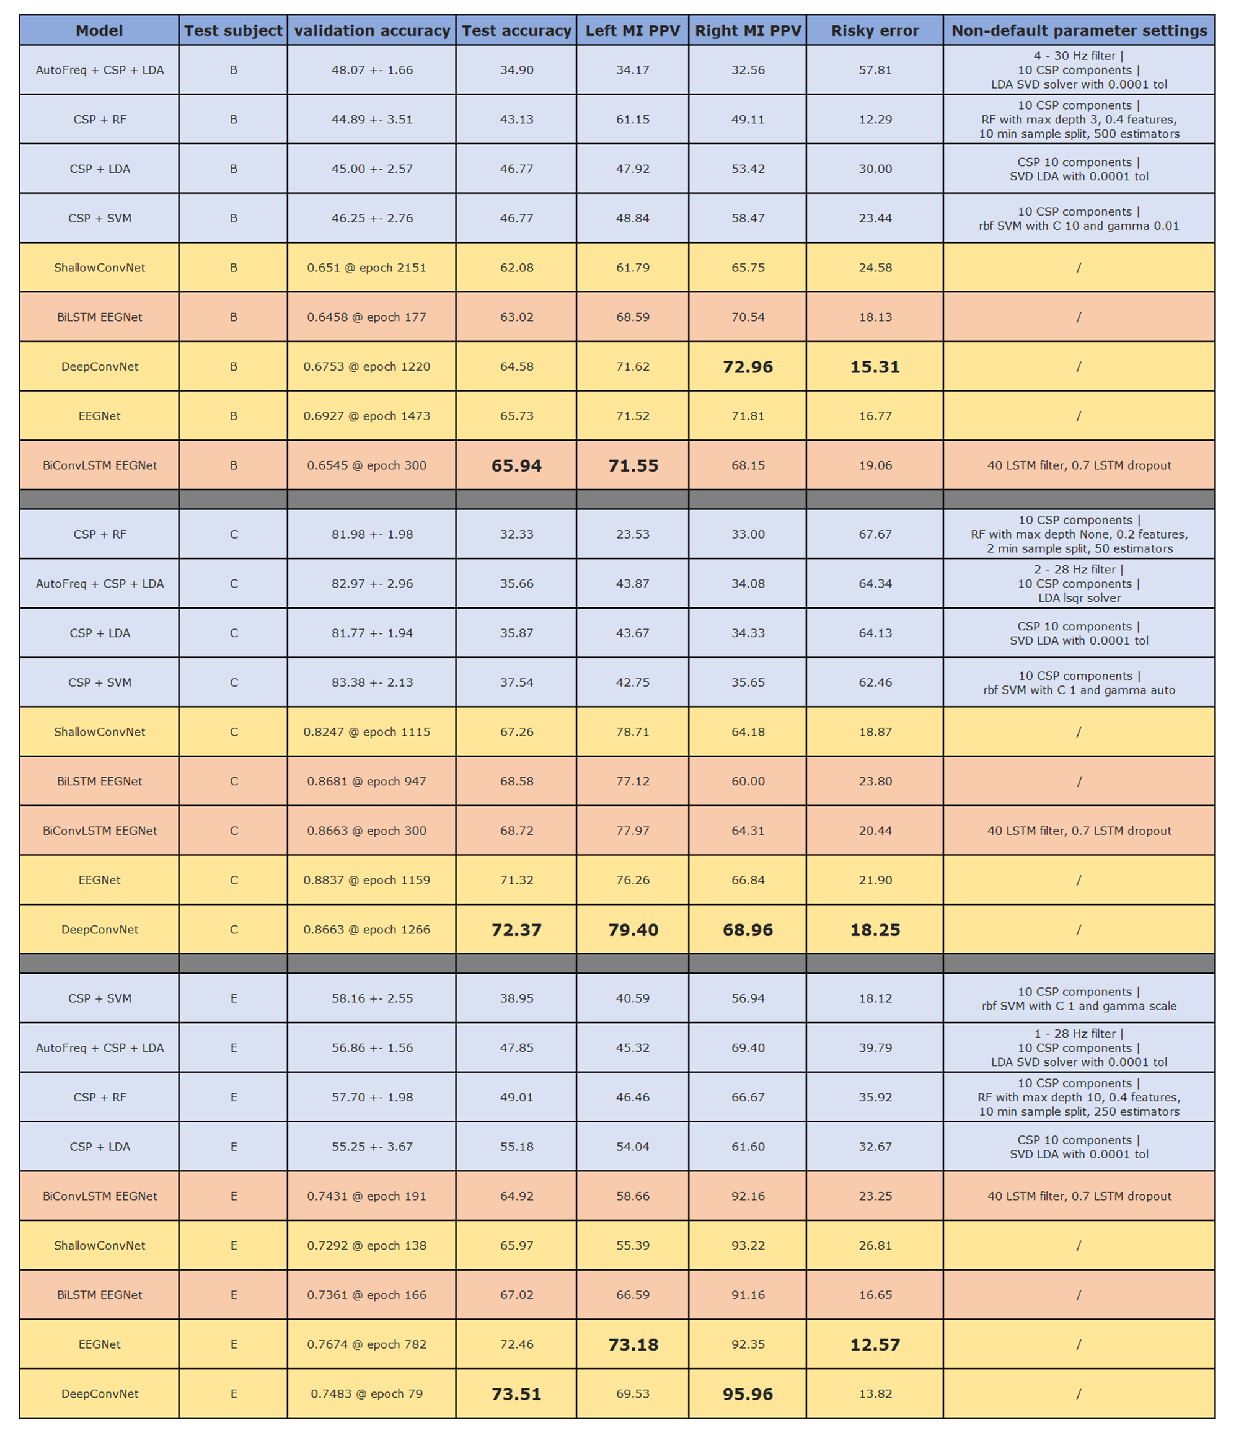
\includegraphics[width=\linewidth]{../images/results/intersession.pdf}
    \captionsetup{width=\linewidth}
    \captionsetup{justification=centering}
    \caption{Intersession results for all classification approaches. Results are sorted based on the test subject and the obtained classification result on the test set. Color coded to denote either two-step \gls{csp} approaches, literature proposed \gls{cnn} approaches and master thesis proposed \gls{cnn}-\gls{lstm} approaches} 
    \label{fig:results_intersession}
\end{figure}




% ---------------------------------------------- 
% INTER SUBJECT
% ---------------------------------------------- 
\section{Intersubject evaluation}
\label{sec:evaluation_intersubject}


\begin{figure}[ht]
    \centering
    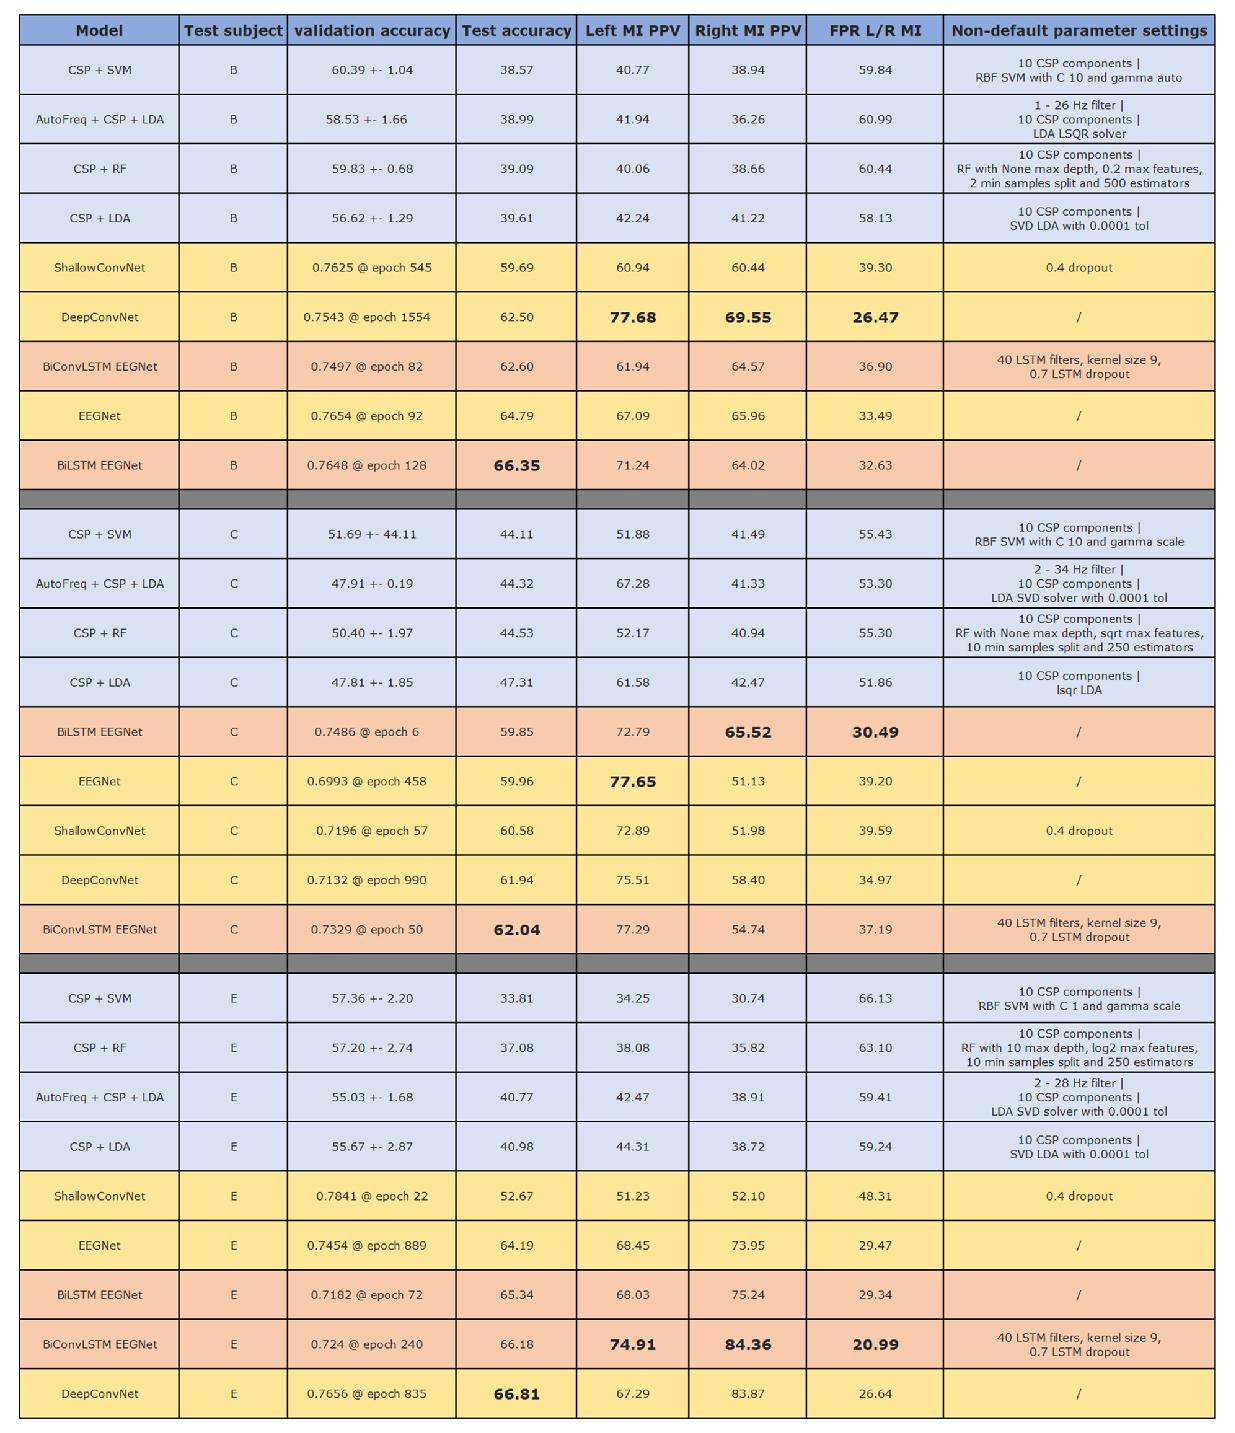
\includegraphics[width=\linewidth]{../images/results/intersubject.pdf}
    \captionsetup{width=\linewidth}
    \captionsetup{justification=centering}
    \caption{Intersubject results for all classification approaches. Results are sorted based on the test subject and the obtained classification result on the test set. Color coded to denote either two-step \gls{csp} approaches, literature proposed \gls{cnn} approaches and master thesis proposed \gls{cnn}-\gls{lstm} approaches} 
    \label{fig:results_intersubject}
\end{figure}


TODO

% ---------------------------------------------- 
% PILOT STUDIES
% ---------------------------------------------- 
\section{Additional pilot studies}
\label{sec:evaluation_pilot_studies}

TODO

% - - - - - - - - - -
% more data
% - - - - - - - - - -
\subsection{Improving intersubject performance by providing more data}
\label{subsec:evaluation_pilot_studies_more data}


TODO

% - - - - - - - - - -
% dropping electrodes
% - - - - - - - - - -
\subsection{Reducing complexity by subsampling the electrodes}
\label{subsec:evaluation_pilot_studies_electrode_drop}


TODO

% - - - - - - - - - -
% calibration
% - - - - - - - - - -
\subsection{Additional finetuning through minimal calibration}
\label{subsec:evaluation_pilot_studies_calibration}


TODO

% - - - - - - - - - -
% prediction time
% - - - - - - - - - -
\subsection{Comparison of prediction times}
\label{subsec:evaluation_pilot_studies_prediction_time}


TODO

% ---------------------------------------------- 
% Conclusions
% ---------------------------------------------- 
\section{Chapter conclusions}
\label{sec:evaluation_conclusions}

TODO
